\documentclass{beamer}

\mode<presentation>
{
  \usetheme{Madrid}   % Copenhagen is sz�p
  \setbeamercovered{transparent}
}
\usepackage{etex}   % a dimenzi�s hiba kisz�r�s�re
\usepackage[magyar]{babel}
\usepackage[latin2]{inputenc}
\usepackage{amssymb}
\usepackage{amsmath}
\usepackage{amscd}
\usepackage{array}
\usepackage{cancel}
\usepackage{color}
\usepackage{enumerate}
\usepackage{epstopdf} 
\usepackage[mathscr]{eucal}
\usepackage[T1]{fontenc}
\usepackage{graphicx}
\usepackage{graphics}
\usepackage{makecell} %vastag vonalak
\usepackage{multirow}
\usepackage{paralist}
\usepackage{ragged2e}
\usepackage{tabularx}
\usepackage{times}
\usepackage{t1enc}

\usepackage[all]{xy}
\usepackage{url}  
\usepackage{xcolor}
\usepackage{framed}

\usepackage{tikz}
\usetikzlibrary{arrows.meta}
\usetikzlibrary{decorations.pathreplacing}

\newcounter{eafel}
\setcounter{eafel}{0}
\newenvironment*{eafela}{ E\textbf{\stepcounter{eafel}\arabic{eafel}.)}}{ }
\resetcounteronoverlays{eafel}

%\newcommand{\defi}[1]{ \vspace{2mm} \textit{Defin�ci�.} \textbf{#1} }
%\newcommand{\tetel}[1]{ \vspace{2mm} \textit{T�tel.} \textbf{#1} }
%\newcommand{\all}{ \vspace{2mm} \textit{�ll�t�s.}  }
\newcommand{\bit}{ \begin{compactitem}}
\newcommand{\eit}{ \end{compactitem} }
\newcommand{\ben}{ \begin{compactenum}[a.)]}
\newcommand{\een}{ \end{compactenum} }
%\renewcommand{\labelitemii}{$\cdot$}
\setdefaultleftmargin{5mm}{2mm}{2mm}{2mm}{2mm}{2mm}
\newcommand{\hely}{\vspace{2mm}}
\newcommand{\kov}{\quad $\Rightarrow$ \quad}
\newcolumntype{M}[1]{>{\centering\arraybackslash}m{#1}}
\renewcommand{\vec}[1]{\boldsymbol{\mathrm{#1}}}
\newcommand{\varr}{\! V\! \! A\! R}
\newcommand{\vava}{\boldsymbol{\vartheta}}

\newcommand{\propnumber}{} % initialize
\newtheorem*{prop}{\propnumber �ll�t�s}
\newenvironment{propc}[1]{\renewcommand{\propnumber}{#1}\begin{prop}}{\end{prop}}
\newcommand{\thnumber}{} % initialize
\newtheorem*{tetel}{\thnumber t�tel}
\newenvironment{tetelc}[1]{\renewcommand{\thnumber}{#1}\begin{tetel}}{\end{tetel}}
\newcommand{\conjnumber}{} % initialize
\newtheorem*{conj}{\conjnumber sejt�s}
\newenvironment{conjc}[1]{\renewcommand{\conjnumber}{#1}\begin{conj}}{\end{conj}}

\title[Pricing APOs] 
{Pricing Average Price Options}

\author[L�szl� Varga] 
{\textbf{L�szl� Varga}}
 
\institute[Citi] 
{
 MQA, Citi
}

\date[Citi FinMath Course] 
{Citi FinMath Course  \\[5mm]
Month Day, Year }


\AtBeginSubsection[]
{
  \begin{frame}<beamer>{Outline}
    \tableofcontents[currentsection,currentsubsection]
  \end{frame}
}


\begin{document}

\begin{frame}
  \titlepage
\end{frame}

\begin{frame}{Outline}
\justifying
  \tableofcontents
\end{frame}

%\section{T�zisek} 

\section{Introduction}

\begin{frame}{Introduction -- average price options}
\justifying
Average price options (APOs) or Asian options: 
\begin{itemize}
\justifying
 \item Derivative contracts written on an average price
 \item Average price: arithmetic or geometric
 \item Usually European style
 \item First appearance: 1987 Tokyo
 \item Advantages:
  \begin{itemize}
  \item smooths volatile market movements
  \item excellent hedging tools when the market participants are exposed to average prices -- popular in commodity markets
 \end{itemize}
 \pause
 \item Pricing methods:
 \begin{itemize}
  \item exact calculation: not always possible or extremely computing intensive
  \item \textbf{moment matching} -- most popular
  \item upper/lower price bounds
  \item numerical solution of the pricing PDE
  \item transformations (Laplace)
  \item Monte Carlo simulation
 \end{itemize}
\end{itemize}
\end{frame}


\begin{frame}{Introduction -- APO types}
\justifying
Payoff of the different European Call APOs: \\[3mm]

\begin{tabular}{l|cc}
Averaging type & Continuously monitored & Discretely monitored \\
\hline
Geometric & $\left( \exp\left\{ \frac{1}{T}\int\limits_0^T \log (S_t)\, dt \right\} \!-\!K \right)_{\!+}$  & $\left(  \left( \prod\limits_{i=1}^n S_{t_i} \right)^{1/n} -K \right)_{\!+}$ \\ \hline
Arithmetic & $\left( \frac{1}{T}\int\limits_0^T S_t\, dt-K \right)_+$  &  $\left( \frac{1}{n} \sum\limits_{i=1}^n S_{t_i} -K \right)_+$
\end{tabular} \\[2mm]
where
 \begin{itemize}
  \item $(S_t)_{t\in [0,T]}$: asset price process
  \item $\{ t_1,\ldots,t_n \}$: fix observation times, $0\leq t_1 \leq \ldots \leq t_n \leq T$ 
  \item $T$: exercise date
  \item $K$: strike
 \end{itemize}
\end{frame}

\section{Commodity APOs and their pricing}

\subsection{Commodity APOs}
 
\begin{frame}{Commodity APOs}
Payoff of the European APO for commodity underlyings:
\begin{equation*}
\text{Payout}_{\text{APO}} = \left( \theta \left( \frac{1}{n}\sum\limits_{i=1}^n F(t_i,T(t_i)) -K \right)  \right)_+
\end{equation*}
where
 \begin{itemize}
  \item $\theta$: $+1$ for call, $-1$ for put options
  \item $n$: total number of averaging days
  \item $\{ t_1,\ldots,t_n \}$: averaging days, usually consecutive
  \item $T(\cdot)$: function, mapping the maturity of the front month contract to the time input
  \item $F(t_i,\tau)$: closing forward price on date $t_i$ for a commodity contract maturing at $\tau$ 
 \end{itemize}
\end{frame}

\begin{frame}{Commodity APOs}
For most products the averaging period is 1 month that covers 2 adjacent futures contracts with maturities $T^{(1)}$ and $T^{(2)}$
\begin{equation*}
\sum\limits_{i=1}^n F(t_i,T(t_i))  = \sum\limits_{i=1}^{n^{(1)}} F(t_i,T^{(1)}) +  \sum\limits_{i=n^{(1)}+1}^n F(t_i,T^{(2)})) 
\end{equation*}
where  $n^{(1)}$ is the rollover day -- last day when the first contract is the front contract: $n^{(1)} = \max \ \{i \in \mathbb{Z}: T(t_i) = T^{(1)}\}$

\vspace{5mm}
\begin{center}
\begin{tikzpicture}
\draw (0,1) -> (12,1);
\draw (1,0.9) -> (1,1.1); \node at (1.05,0.65) {$t_1$};
\draw (2,0.9) -> (2,1.1); \node at (2.05,0.65) {$t_2$};
\draw (3,0.9) -> (3,1.1); \node at (3.05,0.65) {$t_3$};
\node at (4.05,0.65) {$\ldots$};
\draw (5,0.9) -> (5,1.1); \node at (5.05,0.65) {$t_{n^{(1)}}$};
\draw[thick, fill=black] (5.95,0.95) rectangle (6.05,1.05); 
\node at (6.05,0.65) {$T^{(1)}$};
\node at (7.05,0.65) {$\ldots$};
\draw (8,0.9) -> (8,1.1); \node at (8.05,0.65) {$t_{n-1}$};
\draw (9,0.9) -> (9,1.1); \node at (9.05,0.65) {$t_n$};
\draw[thick, fill=black] (10.95,0.95) rectangle (11.05,1.05); 
\node at (11.05,0.65) {$T^{(2)}$};
\end{tikzpicture}
\end{center}

\end{frame}

\subsection{Preliminary results and assumptions}

\begin{frame}{Black '76 formula}
Black-Scholes model in case the underlying is a forward contract \\[2mm]
Notations: \\
 \begin{tabular}{lll}
  $t$ & valuation date \\
  $T$ & option expiry \\
  $T^*$ & forward contract expiry &  $t\leq T \leq T^*$ \\
  $r$ & interest rate \\
  $D_T=e^{-r(T-t)}$ & discount factor  \\
  $F_{t,T} = D_{T} S_t $ & forward price
 \end{tabular} \\[2mm]

Forward price dynamics: $dF_{t,T} = F_{t,T} \sigma \, dW_t$ \quad $\leadsto$\ GBM \\[2mm]
Price of the European call option at time $t$:
\begin{flalign*}
\text{Black}_{\text{Call}}(t,F_{t,T},K, \sigma\sqrt{T},D_{T^*}) &:= D_{T^*}\left[ F_{t,T}\Phi(d_+)-K\Phi(d_-) \right], \text{where} \\
d_{\pm} &= \frac{\log\left( \frac{F_{t,T}}{K} \right) \pm \frac{1}{2}\sigma^2(T-t) }{\sigma \sqrt{T-t}}
\end{flalign*}
\end{frame}

\begin{frame}{Black '76 formula}
What happens with the option price if $\frac{F_{t,T}}{K}<0$ \quad $\Longleftrightarrow$ \quad $F_{t,T}<0$?
\vfill
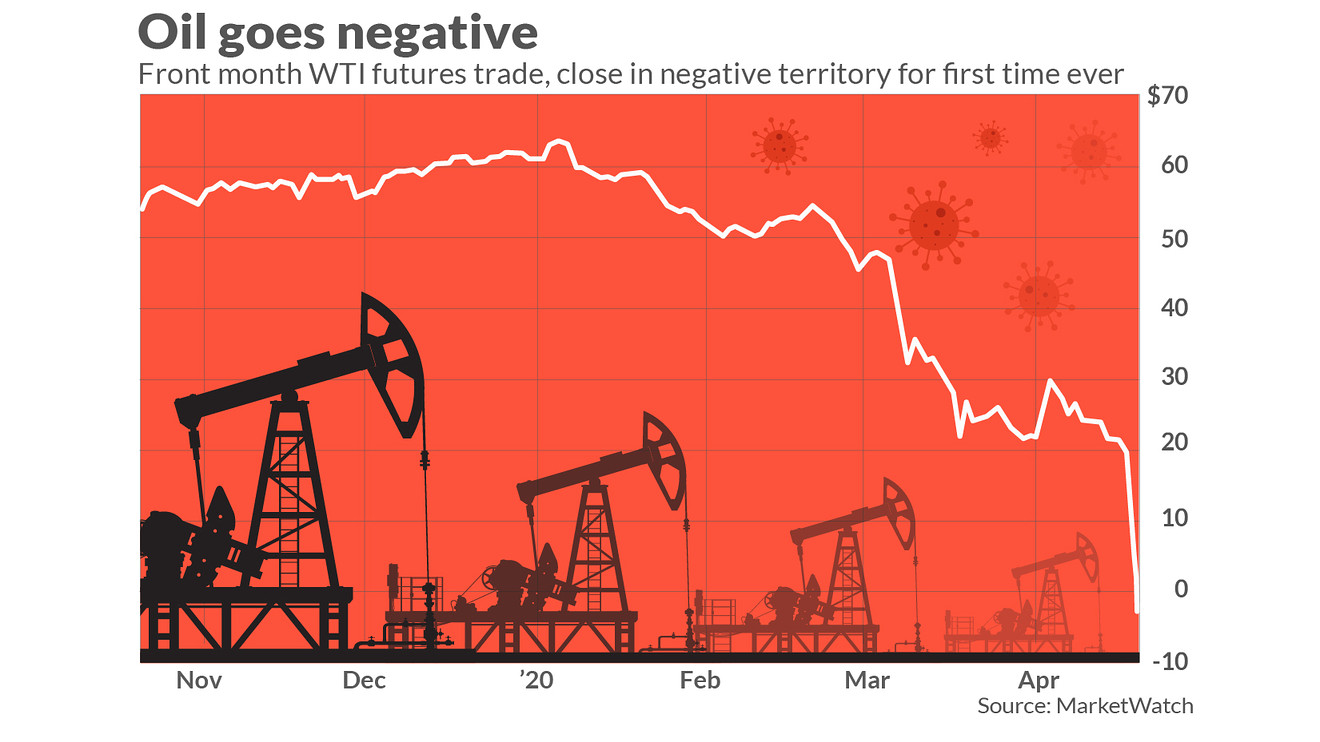
\includegraphics[width=65mm]{OilNeg2.jpg}
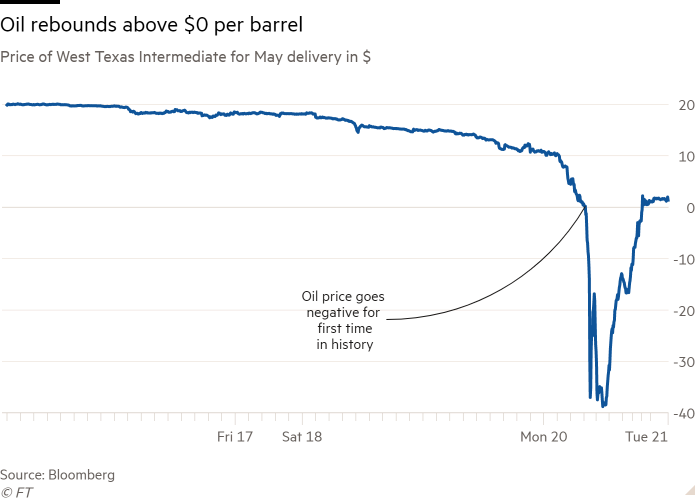
\includegraphics[width=50mm]{OilNeg.png}
\vfill
\pause
Possible remediation: Option price = intrinsic value $= (F_{t,T}-K)_+ $
\end{frame}

\begin{frame}{Averaging method and conventions}
Average price we concentrate on: $V:=\sum\limits_{i=1}^n \omega_i F(t_i,T_i)$, where
\begin{itemize}
 \item $\omega_i$: weights, for APOs \ $\omega_i=\frac{1}{n}$
 \item $T_i:=T(t_i)$
 \item $t$: valuation date
\begin{itemize}
 \item usually $t<t_1\leq \ldots \leq t_n$
 \item if $t>t_1$, then some prices are already known and can be handled as deterministic
\end{itemize}
\end{itemize}
\pause
\vfill
Conventions:
\begin{itemize}
 \item Short duration APO (SD APO): averaging period is at most 1 month 
 \item Long duration APO (LD APO): averaging period is longer than 1 month 
 \item averaging days are weekdays
\end{itemize}
\end{frame}

\begin{frame}{Forward price dynamics}

Multivariate lognormal dynamics:
\begin{flalign*}
dF(t,T_i) &= \sigma(t,T_i)F(t,T_i))\, dW_t^{(i)} \qquad i=1,\ldots,n \\
[W^{(i)},W^{(j)}]_t &= \rho_{i,j}t   \hspace{35mm} i,j=1,\ldots,n 
\end{flalign*}
where $\sigma(t,T_i)=\sigma_i(t)$ is
\begin{itemize}
 \item deterministic
 \item called \textit{instantaneous volatility} of the contract maturing at $T_i$
\end{itemize}

\vfill
\pause
Corollary:
\begin{itemize}
 \item $F(t,T_i)$ has the martingale property
 \item If $t<t_i$, then $F(t_i,T_i) = F(t,T_i) \exp\left\{ -\frac{1}{2}\int\limits_t^{t_i}\sigma_i^2(u)du + \int\limits_t^{t_i}\sigma_i(u)dW^{(i)}(u) \right\} $
\end{itemize}
\end{frame}

\begin{frame}{Models for the volatility}
Instantaneous volatility models -- strike dependence:
\begin{enumerate}
\item Flat model: $\sigma_{i,K}(u)=C_{i,K}\geq 0$ \quad $\forall u \in [t,T_i]$ \quad $\forall i$
\item Samuelson model: $\sigma_{i,K}(u)=C_{i,K}(\sigma_L+e^{-\beta(T_i-u)}) $ \quad $\forall u \in [t,T_i]$ \ $\forall i$
 \begin{itemize}
  \item $\sigma_L$ and $\beta$ are the Samuelson parameters
  \item volatility increases if we get closer to the expiry date 
 \end{itemize}
\end{enumerate}
\vfill
Problem: the instantaneous volatility is not observable on the market, only \textit{implied volatilites} can be obtained as average values:
$$ \widetilde{\sigma}_{i,K}(t) = \sqrt{\frac{1}{T_i-t}\int\limits_t^{T_i}\sigma^2_{i,K}(u)du }
$$
\vfill
For the flat case it is easy to see that $ \widetilde{\sigma}_{i,K}(t)=C_{i,K}$
\vfill
We have 3 different feeder models for the volatility than incorporate volatility smile.
\end{frame}

\begin{frame}{Correlation structure - hyperbolic secant model}
\begin{minipage}{60mm}
$$ \text{sech}(x) =\frac{1}{\text{cosh}(x)}= \frac{2}{e^x+e^{-x}}  $$
\end{minipage}
\begin{minipage}{50mm}
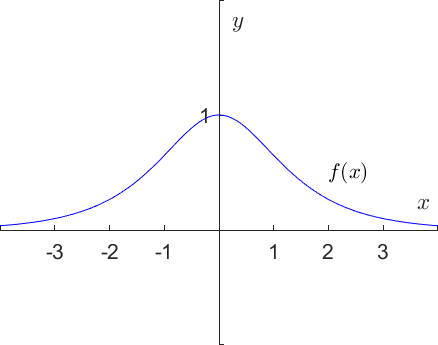
\includegraphics[width=60mm]{sech.png}
\end{minipage}
\vfill
Correlation between two forward contracts: 
\begin{flalign*}
\rho_{i,j} = sech\left( \sqrt{2(1-\rho)}(T_i-T_j) \right) 
\end{flalign*}
where $\rho$ is the so-called \textit{nearby cross-contract correlation} parameter which is calibrated to asset classes
\end{frame}

\subsection{Moment matching}

\begin{frame}{Moment matching -- L�vy approximation}
\begin{itemize}
 \item First proposed by L�vy for Asian options
 \item Payoff of the European call option: $(V-K)_+$, where $V$ is unknown
 \item $M_i = EV^i$ is the $i$th moment of $V$
 \item We approximate $V$ with lognormal distribution which is determined by its first two moments
\end{itemize} 
$$ V \approx F_T = F_0 e^{-\frac{\sigma^2T}{2}+\sigma W_T} $$
\vfill
\begin{tabular}{ll}
Corollary: & $EF_T = F_0 e^{-\frac{\sigma^2T}{2}}E(e^{\sigma W_T}) = 
F_0 e^{-\frac{\sigma^2T}{2}} e^{\frac{\sigma^2T}{2}} = F_0$ \\
& $EF_T^2 = F_0^2 e^{-\sigma^2T} E(e^{2\sigma W_T}) = 
F_0^2 e^{-\sigma^2T} e^{\frac{4\sigma^2T}{2}} = F_0^2 e^{\sigma^2T}$ 
\end{tabular}
\vfill
\begin{minipage}{33mm}
Moment equations:
\end{minipage}
\begin{minipage}{30mm}
\begin{flalign*}
M_1 = EF_T \\
M_2 = EF_T^2 
\end{flalign*}
\end{minipage}
\begin{minipage}{10mm}
$\Longrightarrow$
\end{minipage}
\begin{minipage}{30mm}
\begin{flalign*}
\widehat{F_0} &= M_1  \\
\widehat{\sigma \sqrt{T}} &= \sqrt{\log \left( \frac{M_2}{(M_1)^2} \right)}  
\end{flalign*}
\end{minipage}

Price of the option: $\text{Black}_{\text{Call}}(0, \widehat{F_0},K, \widehat{\sigma \sqrt{T}},D_{T^*}) $
\end{frame}

\begin{frame}{Moment matching -- moments calculation}
Turnbull and Wakeman used this moment matching methodology for the first time for pricing APOs on futures in 1991.

$$ M_1=E_t V = \sum\limits_{i=1}^n \omega_i E_t F(t_i,T_i) =  \sum\limits_{i=1}^n \omega_i F(t,T_i) $$

\begin{flalign*}
M_2 &= E_t V^2 =  \sum\limits_{i=1}^n  \sum\limits_{j=1}^n \omega_i \omega_j 
\underbrace{E_t [F(t_i,T_i) F(t_j,T_j)]}_{E_t [F(t_i,T_i) E_{t_i}F(t_j,T_j) ]} = \\
 &= \sum\limits_{i,j=1}^n \omega_i \omega_j E_t [F(t_i,T_i) F(t_i,T_j)] 
\end{flalign*}
\end{frame}

\begin{frame}{Moment matching -- calculation of $M_2$}
\begin{flalign*}
M_2 &= \sum\limits_{i,j=1}^n \omega_i \omega_j F(t,T_i) F(t,T_j) \exp\left\{ -\frac{1}{2}\int\limits_t^{t_i}(\sigma_i^2(u)+\sigma_j^2(u))du \right\} \cdot \\
 & \qquad \cdot  \underbrace{E_t\left[exp\left\{ \int\limits_t^{t_i} \sigma_i(u) dW^{(i)}(u) + \int\limits_t^{t_i} \sigma_j(u) dW^{(j)}(u)  \right\} \right] }_{E_t\left( e^{X_i+X_j}\right) = e^{0+\frac{1}{2}D^2(X_i+X_j)}= e^{\frac{1}{2} \left(D^2 X_i+D^2X_j+2Cov(X_i,X_j)\right)} }
\end{flalign*}
$X_i:=\int\limits_t^{t_i} \sigma_i(u) dW^{(i)}(u) $ is a stochastic integral with deterministic $\sigma_i$ function, therefore $(X_i,X_j)$ is jointly Gaussian with $EX_i=0$,
 $D^2X_i = \int\limits_t^{t_i} \sigma_i^2(u) du$ \quad and \quad 
 $Cov(X_i,X_j) = \int\limits_t^{t_i} \sigma_i(u)\sigma_j(u) \rho_{i,j} du $.
\end{frame}

\begin{frame}{Moment matching -- calculation of $M_2$}
\begin{flalign*}
M_2 &= \sum\limits_{i,j=1}^n \omega_i \omega_j F(t,T_i) F(t,T_j) \exp\left\{ \rho_{i,j} \int\limits_t^{t_i} \sigma_i(u)\sigma_j(u)  du\right\} 
\end{flalign*}
For the flat volatility model we have
\begin{flalign*}
M_2 &= \sum\limits_{i,j=1}^n \omega_i \omega_j F(t,T_i) F(t,T_j) e^{ \rho_{i,j} (t_i-t)C_{i,K}C_{j,K} } 
\end{flalign*}
For the Samuelson volatility model we have
\begin{flalign*}
M_2 &= \sum\limits_{i,j=1}^n \omega_i \omega_j F(t,T_i) F(t,T_j) \exp\left\{ \rho_{i,j} A_t^{i,j} (t_i-t)\tilde{\sigma}_{i,K}(t) \tilde{\sigma}_{j,K}(t) \right\} 
\end{flalign*}
where $A_t^{i,j}$ has an explicit, but very long form.
\end{frame}

\section{Conclusions}

\begin{frame}{Conclusions}
Experience with the moment matching technique
\begin{itemize}
 \item Model in 10+ years' use
 \item The approximation is very good for SD APOs, somewhat worse for LD APOs
 \item The approximation gets worse the later the averaging period starts
 \item Fast calculations
 \item Independent Excel implementation: even the largest differences are only of $10^{-8}$ magnitude
 \item Risk are stable even under severely stressed conditions
 \item Benchmark with 4 moment matching -- not much better
 \item Certain parameters are not enough frequently calibrated
 \item Risk sensitivities are not stable if prices go negative even with the intrinsic value usage
\end{itemize}
\end{frame}


%%%%%%%%%%%%%%%%%%%%%%%%%%%%%%%%%%%%%%%%%%%%%%%%%%%%%%%%%%%%%%%%%%%%%%%%%%%%%%%%%%%%%%%%%%

\begin{frame}{}
\centering
\LARGE
Thank you for the attention!
\vfill
Questions / comments?
\vfill
\vfill
%\large
%Acknowledgement: D�niel Di�s and K�lm�n Cziszter
\end{frame}

\begin{frame}{References}
 \begin{itemize}
  \item Stuart M. Turnbull and Lee MacDonald Wakeman: A Quick Algorithm for Pricing European Average Options. \\ The Journal of Financial and Quantitative Analysis \\
Vol. 26, No. 3 (Sep., 1991), pp. 377-389 \\ \textit{Cambridge University Press}
 \item Roncoroni, A. and Fusai, G. and Cummins, M. (2015): Handbook of multi-commodity markets and products: Structuring, trading and risk management. \\ Chapter 18 (p. 827-877), \textit{John Wiley \& Sons} 
 \end{itemize}
\end{frame}

\end{document}
